\documentclass[twoside]{book}

% Packages required by doxygen
\usepackage{fixltx2e}
\usepackage{calc}
\usepackage{doxygen}
\usepackage[export]{adjustbox} % also loads graphicx
\usepackage{graphicx}
\usepackage[utf8]{inputenc}
\usepackage{makeidx}
\usepackage{multicol}
\usepackage{multirow}
\PassOptionsToPackage{warn}{textcomp}
\usepackage{textcomp}
\usepackage[nointegrals]{wasysym}
\usepackage[table]{xcolor}

% Font selection
\usepackage[T1]{fontenc}
\usepackage[scaled=.90]{helvet}
\usepackage{courier}
\usepackage{amssymb}
\usepackage{sectsty}
\renewcommand{\familydefault}{\sfdefault}
\allsectionsfont{%
  \fontseries{bc}\selectfont%
  \color{darkgray}%
}
\renewcommand{\DoxyLabelFont}{%
  \fontseries{bc}\selectfont%
  \color{darkgray}%
}
\newcommand{\+}{\discretionary{\mbox{\scriptsize$\hookleftarrow$}}{}{}}

% Page & text layout
\usepackage{geometry}
\geometry{%
  a4paper,%
  top=2.5cm,%
  bottom=2.5cm,%
  left=2.5cm,%
  right=2.5cm%
}
\tolerance=750
\hfuzz=15pt
\hbadness=750
\setlength{\emergencystretch}{15pt}
\setlength{\parindent}{0cm}
\setlength{\parskip}{3ex plus 2ex minus 2ex}
\makeatletter
\renewcommand{\paragraph}{%
  \@startsection{paragraph}{4}{0ex}{-1.0ex}{1.0ex}{%
    \normalfont\normalsize\bfseries\SS@parafont%
  }%
}
\renewcommand{\subparagraph}{%
  \@startsection{subparagraph}{5}{0ex}{-1.0ex}{1.0ex}{%
    \normalfont\normalsize\bfseries\SS@subparafont%
  }%
}
\makeatother

% Headers & footers
\usepackage{fancyhdr}
\pagestyle{fancyplain}
\fancyhead[LE]{\fancyplain{}{\bfseries\thepage}}
\fancyhead[CE]{\fancyplain{}{}}
\fancyhead[RE]{\fancyplain{}{\bfseries\leftmark}}
\fancyhead[LO]{\fancyplain{}{\bfseries\rightmark}}
\fancyhead[CO]{\fancyplain{}{}}
\fancyhead[RO]{\fancyplain{}{\bfseries\thepage}}
\fancyfoot[LE]{\fancyplain{}{}}
\fancyfoot[CE]{\fancyplain{}{}}
\fancyfoot[RE]{\fancyplain{}{\bfseries\scriptsize Generated by Doxygen }}
\fancyfoot[LO]{\fancyplain{}{\bfseries\scriptsize Generated by Doxygen }}
\fancyfoot[CO]{\fancyplain{}{}}
\fancyfoot[RO]{\fancyplain{}{}}
\renewcommand{\footrulewidth}{0.4pt}
\renewcommand{\chaptermark}[1]{%
  \markboth{#1}{}%
}
\renewcommand{\sectionmark}[1]{%
  \markright{\thesection\ #1}%
}

% Indices & bibliography
\usepackage{natbib}
\usepackage[titles]{tocloft}
\setcounter{tocdepth}{3}
\setcounter{secnumdepth}{5}
\makeindex

% Hyperlinks (required, but should be loaded last)
\usepackage{ifpdf}
\ifpdf
  \usepackage[pdftex,pagebackref=true]{hyperref}
\else
  \usepackage[ps2pdf,pagebackref=true]{hyperref}
\fi
\hypersetup{%
  colorlinks=true,%
  linkcolor=blue,%
  citecolor=blue,%
  unicode%
}

% Custom commands
\newcommand{\clearemptydoublepage}{%
  \newpage{\pagestyle{empty}\cleardoublepage}%
}

\usepackage{caption}
\captionsetup{labelsep=space,justification=centering,font={bf},singlelinecheck=off,skip=4pt,position=top}

%===== C O N T E N T S =====

\begin{document}

% Titlepage & ToC
\hypersetup{pageanchor=false,
             bookmarksnumbered=true,
             pdfencoding=unicode
            }
\pagenumbering{alph}
\begin{titlepage}
\vspace*{7cm}
\begin{center}%
{\Large My Project }\\
\vspace*{1cm}
{\large Generated by Doxygen 1.8.13}\\
\end{center}
\end{titlepage}
\clearemptydoublepage
\pagenumbering{roman}
\tableofcontents
\clearemptydoublepage
\pagenumbering{arabic}
\hypersetup{pageanchor=true}

%--- Begin generated contents ---
\chapter{The Canny Edge Detection Project}
\label{index}\hypertarget{index}{}\hypertarget{index_intro_sec}{}\section{Introduction}\label{index_intro_sec}
Canny edge detection is a multi-\/step image filter that detects only the outlines of an image. It is the culmination of 6 individual filters, applied one after another until only the edges of the original image are pronounced.\hypertarget{index_how_works_sec}{}\section{How it Works\+:}\label{index_how_works_sec}
Each of the below filters are applied to an image. Starting with a Greyscale \hyperlink{classFilter}{Filter} and ending with a Hysteresis \hyperlink{classFilter}{Filter}. The resulting image is a Canny Edge Detection Filtered image.


\begin{DoxyEnumerate}
\item Greyscale
\item Gaussian blur
\item Sobel filter
\item Non-\/max suppression
\item Double threshold
\item Hysteresis
\end{DoxyEnumerate}
\chapter{Hierarchical Index}
\section{Class Hierarchy}
This inheritance list is sorted roughly, but not completely, alphabetically\+:\begin{DoxyCompactList}
\item \contentsline{section}{Filter}{\pageref{classFilter}}{}
\begin{DoxyCompactList}
\item \contentsline{section}{Double\+Threshold\+Filter}{\pageref{classDoubleThresholdFilter}}{}
\item \contentsline{section}{Grey\+Scale\+Filter}{\pageref{classGreyScaleFilter}}{}
\item \contentsline{section}{Hysteresis\+Filter}{\pageref{classHysteresisFilter}}{}
\end{DoxyCompactList}
\item \contentsline{section}{Image}{\pageref{classImage}}{}
\item \contentsline{section}{stbi\+\_\+io\+\_\+callbacks}{\pageref{structstbi__io__callbacks}}{}
\end{DoxyCompactList}

\chapter{Class Index}
\section{Class List}
Here are the classes, structs, unions and interfaces with brief descriptions\+:\begin{DoxyCompactList}
\item\contentsline{section}{\hyperlink{classBeeline}{Beeline} \\*The class for moving the drone in a straight line from point A to point B }{\pageref{classBeeline}}{}
\item\contentsline{section}{\hyperlink{classDrone}{Drone} \\*The class for representing the drone object in the simulation }{\pageref{classDrone}}{}
\item\contentsline{section}{\hyperlink{classEntityFactory}{Entity\+Factory} \\*The class for creating json object entities }{\pageref{classEntityFactory}}{}
\item\contentsline{section}{\hyperlink{classMovement}{Movement} \\*The class for handling movement of the drone }{\pageref{classMovement}}{}
\item\contentsline{section}{\hyperlink{classSimulation}{Simulation} \\*The class for simulating a drone finding a robot }{\pageref{classSimulation}}{}
\item\contentsline{section}{\hyperlink{classWebApp}{Web\+App} \\*A Web Application Sever that communicates with a web page through web sockets }{\pageref{classWebApp}}{}
\end{DoxyCompactList}

\chapter{Class Documentation}
\hypertarget{classDoubleThresholdFilter}{}\section{Double\+Threshold\+Filter Class Reference}
\label{classDoubleThresholdFilter}\index{Double\+Threshold\+Filter@{Double\+Threshold\+Filter}}


Inheritance diagram for Double\+Threshold\+Filter\+:\nopagebreak
\begin{figure}[H]
\begin{center}
\leavevmode
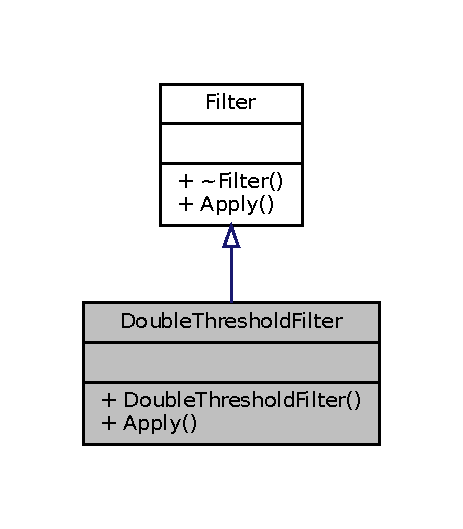
\includegraphics[width=222pt]{classDoubleThresholdFilter__inherit__graph}
\end{center}
\end{figure}


Collaboration diagram for Double\+Threshold\+Filter\+:\nopagebreak
\begin{figure}[H]
\begin{center}
\leavevmode
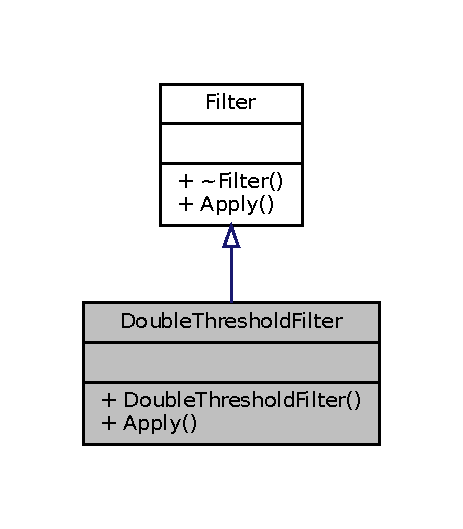
\includegraphics[width=222pt]{classDoubleThresholdFilter__coll__graph}
\end{center}
\end{figure}
\subsection*{Public Member Functions}
\begin{DoxyCompactItemize}
\item 
\mbox{\Hypertarget{classDoubleThresholdFilter_a913781178b551ee558833d1ef207837f}\label{classDoubleThresholdFilter_a913781178b551ee558833d1ef207837f}} 
{\bfseries Double\+Threshold\+Filter} (float h, float l)
\item 
\mbox{\Hypertarget{classDoubleThresholdFilter_aaf926813c03a95d5945625d60a811a3c}\label{classDoubleThresholdFilter_aaf926813c03a95d5945625d60a811a3c}} 
void {\bfseries Apply} (std\+::vector$<$ \hyperlink{classImage}{Image} $\ast$$>$ original, std\+::vector$<$ \hyperlink{classImage}{Image} $\ast$$>$ filtered)
\end{DoxyCompactItemize}


The documentation for this class was generated from the following files\+:\begin{DoxyCompactItemize}
\item 
/home/user/repo/\+Iteration1/src/double-\/threshold.\+h\item 
/home/user/repo/\+Iteration1/src/double-\/threshold.\+cc\end{DoxyCompactItemize}

\hypertarget{classFilter}{}\section{Filter Class Reference}
\label{classFilter}\index{Filter@{Filter}}


Inheritance diagram for Filter\+:\nopagebreak
\begin{figure}[H]
\begin{center}
\leavevmode
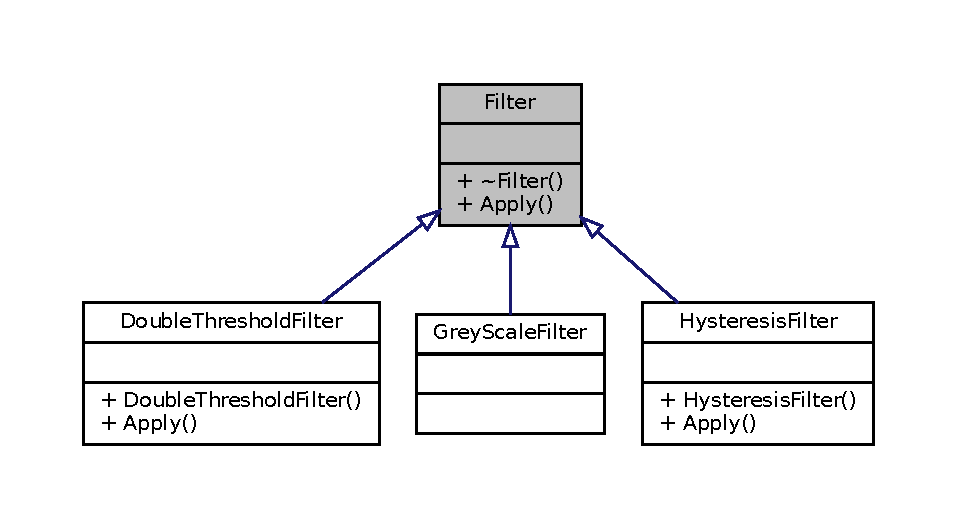
\includegraphics[width=350pt]{classFilter__inherit__graph}
\end{center}
\end{figure}


Collaboration diagram for Filter\+:\nopagebreak
\begin{figure}[H]
\begin{center}
\leavevmode
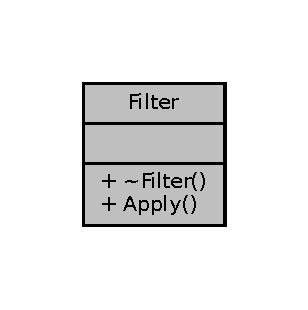
\includegraphics[width=148pt]{classFilter__coll__graph}
\end{center}
\end{figure}
\subsection*{Public Member Functions}
\begin{DoxyCompactItemize}
\item 
\mbox{\Hypertarget{classFilter_afab0d50af44a19a370ebe46c69b8ff4e}\label{classFilter_afab0d50af44a19a370ebe46c69b8ff4e}} 
virtual void {\bfseries Apply} (std\+::vector$<$ \hyperlink{classImage}{Image} $\ast$$>$ original, std\+::vector$<$ \hyperlink{classImage}{Image} $\ast$$>$ filtered)=0
\end{DoxyCompactItemize}


The documentation for this class was generated from the following file\+:\begin{DoxyCompactItemize}
\item 
/home/user/repo/\+Iteration1/src/filter.\+h\end{DoxyCompactItemize}

\hypertarget{classGreyScaleFilter}{}\section{Grey\+Scale\+Filter Class Reference}
\label{classGreyScaleFilter}\index{Grey\+Scale\+Filter@{Grey\+Scale\+Filter}}


Inheritance diagram for Grey\+Scale\+Filter\+:\nopagebreak
\begin{figure}[H]
\begin{center}
\leavevmode
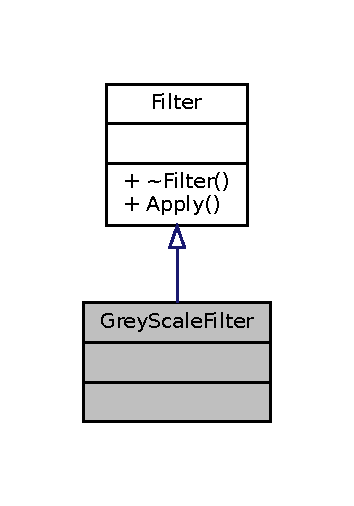
\includegraphics[width=170pt]{classGreyScaleFilter__inherit__graph}
\end{center}
\end{figure}


Collaboration diagram for Grey\+Scale\+Filter\+:\nopagebreak
\begin{figure}[H]
\begin{center}
\leavevmode
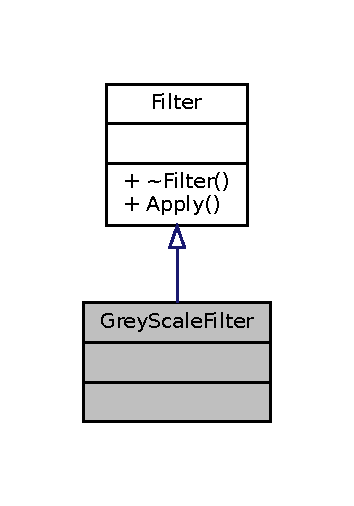
\includegraphics[width=170pt]{classGreyScaleFilter__coll__graph}
\end{center}
\end{figure}
\subsection*{Additional Inherited Members}


The documentation for this class was generated from the following files\+:\begin{DoxyCompactItemize}
\item 
/home/user/repo/\+Iteration1/src/greyscale\+\_\+filter.\+h\item 
/home/user/repo/\+Iteration1/src/greyscale\+\_\+filter.\+cc\end{DoxyCompactItemize}

\hypertarget{classHysteresisFilter}{}\section{Hysteresis\+Filter Class Reference}
\label{classHysteresisFilter}\index{Hysteresis\+Filter@{Hysteresis\+Filter}}


Inheritance diagram for Hysteresis\+Filter\+:\nopagebreak
\begin{figure}[H]
\begin{center}
\leavevmode
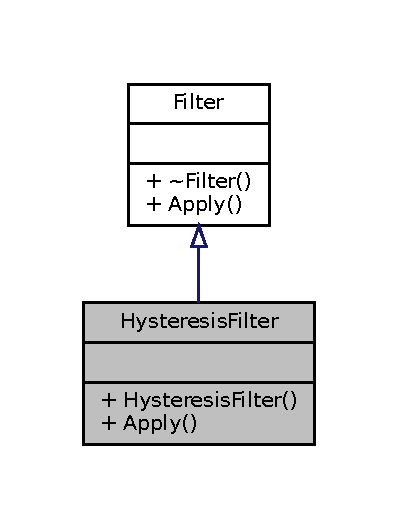
\includegraphics[width=191pt]{classHysteresisFilter__inherit__graph}
\end{center}
\end{figure}


Collaboration diagram for Hysteresis\+Filter\+:\nopagebreak
\begin{figure}[H]
\begin{center}
\leavevmode
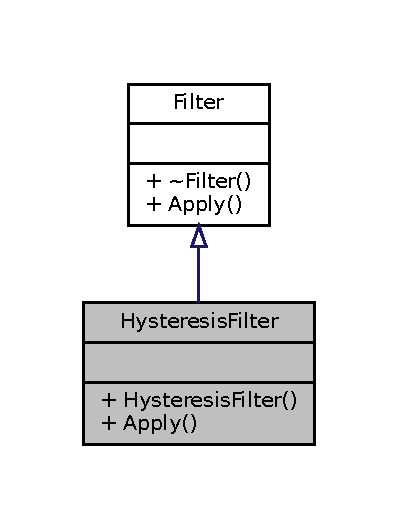
\includegraphics[width=191pt]{classHysteresisFilter__coll__graph}
\end{center}
\end{figure}
\subsection*{Public Member Functions}
\begin{DoxyCompactItemize}
\item 
\mbox{\Hypertarget{classHysteresisFilter_af2d6c50bc0cfd609fbf7e90f01b03b1f}\label{classHysteresisFilter_af2d6c50bc0cfd609fbf7e90f01b03b1f}} 
void {\bfseries Apply} (std\+::vector$<$ \hyperlink{classImage}{Image} $\ast$$>$ original, std\+::vector$<$ \hyperlink{classImage}{Image} $\ast$$>$ filtered)
\end{DoxyCompactItemize}


The documentation for this class was generated from the following files\+:\begin{DoxyCompactItemize}
\item 
/home/user/repo/\+Iteration1/src/hysteresis.\+h\item 
/home/user/repo/\+Iteration1/src/hysteresis.\+cc\end{DoxyCompactItemize}

\hypertarget{classImage}{}\section{Image Class Reference}
\label{classImage}\index{Image@{Image}}


Collaboration diagram for Image\+:\nopagebreak
\begin{figure}[H]
\begin{center}
\leavevmode
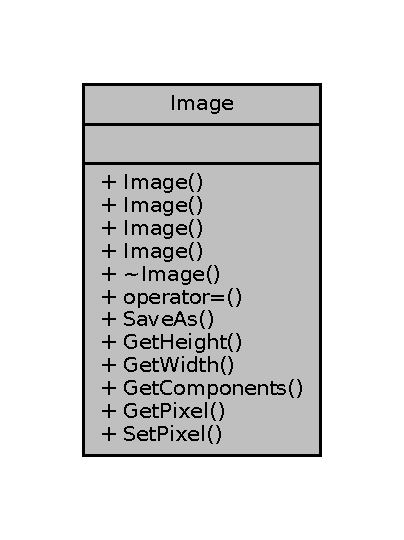
\includegraphics[width=194pt]{classImage__coll__graph}
\end{center}
\end{figure}
\subsection*{Public Member Functions}
\begin{DoxyCompactItemize}
\item 
\mbox{\Hypertarget{classImage_a6383baa72a87f006f0d1ab1ac19006eb}\label{classImage_a6383baa72a87f006f0d1ab1ac19006eb}} 
{\bfseries Image} (int height, int width)
\item 
\mbox{\Hypertarget{classImage_abb20937b3256735f0f7549d1b5e9c10d}\label{classImage_abb20937b3256735f0f7549d1b5e9c10d}} 
{\bfseries Image} (std\+::string filename)
\item 
\mbox{\Hypertarget{classImage_ad06dec9531d61e2fd4c5fa761201bb20}\label{classImage_ad06dec9531d61e2fd4c5fa761201bb20}} 
{\bfseries Image} (const \hyperlink{classImage}{Image} \&vec)
\item 
\mbox{\Hypertarget{classImage_a4da7f72e4063bd0764caa635c0e0aaae}\label{classImage_a4da7f72e4063bd0764caa635c0e0aaae}} 
void {\bfseries operator=} (const \hyperlink{classImage}{Image} \&img)
\item 
\mbox{\Hypertarget{classImage_a3a9b278005e0731a93fe1d5d2cff7104}\label{classImage_a3a9b278005e0731a93fe1d5d2cff7104}} 
void {\bfseries Save\+As} (std\+::string filename)
\item 
\mbox{\Hypertarget{classImage_a631ead4be012caf49b3209d2ac401214}\label{classImage_a631ead4be012caf49b3209d2ac401214}} 
int {\bfseries Get\+Height} () const
\item 
\mbox{\Hypertarget{classImage_a3da5012d5e314ce03b53d77276232186}\label{classImage_a3da5012d5e314ce03b53d77276232186}} 
int {\bfseries Get\+Width} () const
\item 
\mbox{\Hypertarget{classImage_a72295fcd1c416436284a1a8fae68e2f8}\label{classImage_a72295fcd1c416436284a1a8fae68e2f8}} 
int {\bfseries Get\+Components} () const
\item 
\mbox{\Hypertarget{classImage_a5518f009939758554a3177b13414cc68}\label{classImage_a5518f009939758554a3177b13414cc68}} 
Color {\bfseries Get\+Pixel} (int a, int b)
\item 
\mbox{\Hypertarget{classImage_ad8230d239bf601268eda4f0ae757e3c3}\label{classImage_ad8230d239bf601268eda4f0ae757e3c3}} 
void {\bfseries Set\+Pixel} (int a, int b, Color input)
\end{DoxyCompactItemize}


The documentation for this class was generated from the following files\+:\begin{DoxyCompactItemize}
\item 
/home/user/repo/\+Iteration1/src/image.\+h\item 
/home/user/repo/\+Iteration1/src/image.\+cc\end{DoxyCompactItemize}

\hypertarget{structstbi__io__callbacks}{}\section{stbi\+\_\+io\+\_\+callbacks Struct Reference}
\label{structstbi__io__callbacks}\index{stbi\+\_\+io\+\_\+callbacks@{stbi\+\_\+io\+\_\+callbacks}}


Collaboration diagram for stbi\+\_\+io\+\_\+callbacks\+:\nopagebreak
\begin{figure}[H]
\begin{center}
\leavevmode
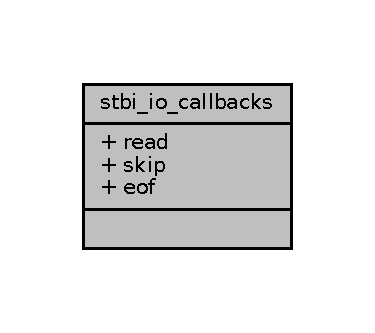
\includegraphics[width=180pt]{structstbi__io__callbacks__coll__graph}
\end{center}
\end{figure}
\subsection*{Public Attributes}
\begin{DoxyCompactItemize}
\item 
\mbox{\Hypertarget{structstbi__io__callbacks_a623e46b3a2a019611601409926283a88}\label{structstbi__io__callbacks_a623e46b3a2a019611601409926283a88}} 
int($\ast$ {\bfseries read} )(void $\ast$user, char $\ast$data, int size)
\item 
\mbox{\Hypertarget{structstbi__io__callbacks_a257aac5480a90a6c4b8fbe86c1b01068}\label{structstbi__io__callbacks_a257aac5480a90a6c4b8fbe86c1b01068}} 
void($\ast$ {\bfseries skip} )(void $\ast$user, int n)
\item 
\mbox{\Hypertarget{structstbi__io__callbacks_a319639db2f76e715eed7a7a974136832}\label{structstbi__io__callbacks_a319639db2f76e715eed7a7a974136832}} 
int($\ast$ {\bfseries eof} )(void $\ast$user)
\end{DoxyCompactItemize}


The documentation for this struct was generated from the following file\+:\begin{DoxyCompactItemize}
\item 
/home/user/repo/\+Iteration1/src/stb\+\_\+image.\+h\end{DoxyCompactItemize}

%--- End generated contents ---

% Index
\backmatter
\newpage
\phantomsection
\clearemptydoublepage
\addcontentsline{toc}{chapter}{Index}
\printindex

\end{document}
